\section{The effect of ageing on turquoise killifish antibody repertoires}
\label{sec:igseq_ageing}

The pilot study into the antibody repertoires of mature adult turquoise killifish (\Cref{sec:igseq_pilot}) demonstrated that... % TODO: Briefly summarise importance of pilot results
However, ... % TODO: Segue into testing across age

In order to investigate the effects of ageing on the killifish antibody repertoire, In order to investigate the effect of ageing on these processes, each of the 32 fish described in  \Cref{tab:igseq-cohorts-summary,tab:igseq-cohorts-fish} % TODO: Figure of age groups? Describe better?
underwent two independent library preparations as described in \Cref{sec:methods_molec_igseq} and \Cref{sec:igseq_protocol_library}, % TODO: Table of cycle numbers etc.
for a total of 64 pooled libraries; these were then sequenced together in two MiSeq runs, yielding a total of \embed{_Figures/txt/ageing-reads-raw-total.txt} million read pairs (\embed{_Figures/txt/ageing-reads-raw-replicate-min.txt} to \embed{_Figures/txt/ageing-reads-raw-replicate-max.txt} million pairs per replicate, \embed{_Figures/txt/ageing-reads-raw-individual-min.txt} to \embed{_Figures/txt/ageing-reads-raw-individual-max.txt} million pairs per individual), and the resulting reads underwent pre-processing, filtering and clonotyping as described in \Cref{sec:igseq_protocol_preprocess,sec:igseq_pilot_composition,sec:igseq_pilot_clones}.

\Cref{fig:igseq-ageing-read-survival-all} shows the absolute and relative read survival for each of the sixty-four sequencing libraries throughout this process. As with the pilot dataset, the replicates show relatively consistent behaviour up to and including VDJ assignment and Change-O database construction, with \embed{_Figures/txt/ageing-read-survival-init-min.txt}\,\% to \embed{_Figures/txt/ageing-read-survival-init-max.txt}\,\% of reads surviving up to this stage in the pipeline. However, a somewhat % TODO: much?
 larger number of sequences (\embed{_Figures/txt/ageing-read-survival-rel-loss-total.txt}\,\%, up to \embed{_Figures/txt/ageing-read-survival-rel-loss-max.txt}\,\% per replicate) are lost during V-score filtering compared to the pilot dataset (\embed{_Figures/txt/pilot-read-survival-rel-loss-total.txt}\,\%, up to \embed{_Figures/txt/pilot-read-survival-rel-loss-max.txt}\,\% per replicate). This inconsistency is due to a greater preponderance in the ageing dataset of malformed, J-identity-lacking sequences, which in this case actually make up an absolute majority of unique sequences in the \program{pRESTO}-processed dataset (\Cref{fig:igseq-ageing-functional-prop-pre}). After filtering on V-score, however, the functional composition of the ageing dataset is similar to that of the pilot data (\Cref{fig:igseq-ageing-functional-prop-post,fig:igseq-pilot-functional-prop-b}).

\begin{figure}
\centering
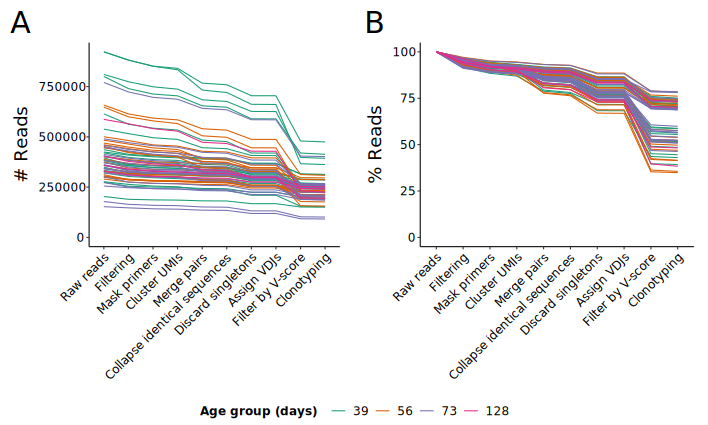
\includegraphics[width = 0.9\textwidth]{_Figures/png/ageing-read-survival-all.png}
\begin{subfigure}{0em}
\phantomsubcaption{}
\label{fig:igseq-ageing-read-survival-all-abs}
\end{subfigure}
\begin{subfigure}{0em}
\phantomsubcaption{}
\label{fig:igseq-ageing-read-survival-all-rel}
\end{subfigure}
\caption{Absolute (A) and relative (B) read survival during pre-processing of the \igseq ageing dataset, up to and including clonotyping.}
\label{fig:igseq-ageing-read-survival-all}
\end{figure}

\begin{figure}
\centering
\includegraphics[width = 0.9\textwidth]{_Figures/png/ageing-functional-prop}
\begin{subfigure}{0em}
\phantomsubcaption{}
\label{fig:igseq-ageing-functional-prop-pre}
\end{subfigure}
\begin{subfigure}{0em}
\phantomsubcaption{}
\label{fig:igseq-ageing-functional-prop-post}
\end{subfigure}
\caption{Proportion of input reads, UMI groups and unique sequences in the \igseq ageing dataset belonging to different (non)functional categories, before (A) and after (B) filtering on V-alignment score.}
\label{fig:igseq-ageing-functional-prop}
\end{figure}

Following V-score filtering, \embed{_Figures/txt/ageing-nseq-assigned-clones.txt}\,\% of remaining unique sequences in the ageing dataset were successfully assigned clonal identities. The number of clones inferred per individual ranged from \embed{_Figures/txt/ageing-nclones-individual-min.txt} to \embed{_Figures/txt/ageing-nclones-individual-max.txt}, with a median of \embed{_Figures/txt/ageing-nclones-individual-med.txt}. This is much lower than the median of \embed{_Figures/txt/pilot-nclones-individual-med.txt} clones per individual for the pilot study, reflecting the lower number of reads per individual available in this dataset; for comparison, for the four individuals included in the pilot study, the number of identified clones in the ageing dataset ranges from \embed{_Figures/txt/ageing-nclones-individual-min-pilot.txt} to \embed{_Figures/txt/ageing-nclones-individual-max-pilot.txt}.
% TODO: Boxplot of clone counts across age groups
Concordantly, the distribution of clone sizes detected is even more skewed towards small clones than in the pilot dataset: \embed{_Figures/txt/ageing-nclones-pc-1count.txt}\,\% of clones are observed as just a single unique sequence across all replicates, while \embed{_Figures/txt/ageing-nclones-pc-small.txt}\,\% contain fewer than five unique sequences (\Cref{fig:igseq-ageing-clone-sizes-sizes}). As in the pilot dataset, larger clones were much more likely to be observed across both replicates for a given individual  (\Cref{fig:igseq-ageing-clone-sizes-reps}).

% TODO: Discuss 700-clone individual as a negative outlier 

% TODO: Discuss inter-replicate correlational pattern
% TODO: Discuss Zipf fit & P20

\begin{figure}
\centering
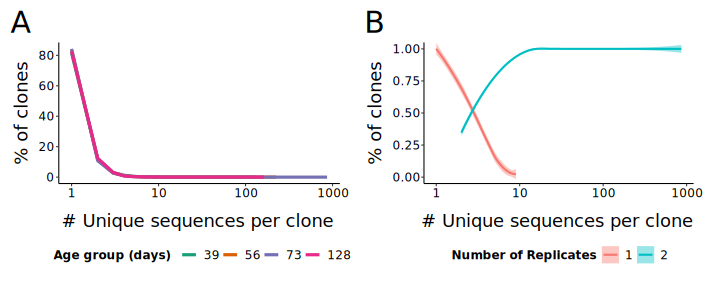
\includegraphics[width = 0.9\textwidth]{_Figures/png/ageing-clone-sizes}
\begin{subfigure}{0em}
\phantomsubcaption{}
\label{fig:igseq-ageing-clone-sizes-sizes}
\end{subfigure}
\begin{subfigure}{0em}
\phantomsubcaption{}
\label{fig:igseq-ageing-clone-sizes-reps}
\end{subfigure}
\caption{(A) Proportion of clones of different sizes for each individual in the ageing dataset, measured in unique sequences per clone. (B) Proportion of clones of each size found across one or both replicates of the appropriate individual.}
% TODO: Add suitable overall figure title
\label{fig:igseq-ageing-clone-sizes}
\end{figure}

\begin{figure}
\centering
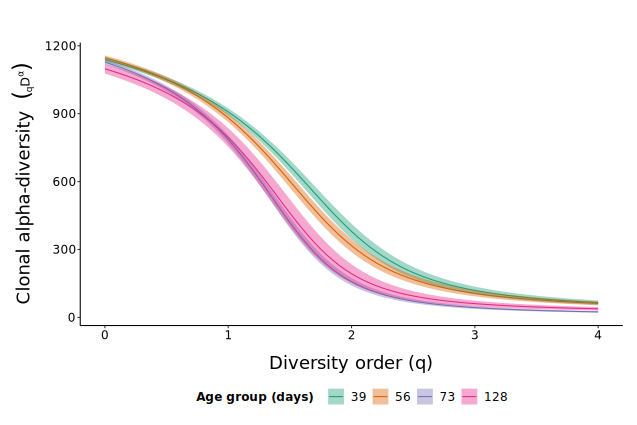
\includegraphics[width = 0.9\textwidth]{_Figures/png/ageing-clone-diversity-alpha}
\caption{\textbf{Killifish alpha-diversity declines with age:} Bootstrapped alpha-diversity spectra of clone sizes for each age group in the \igseq ageing dataset, as measured by number of unique sequences per clone.}
\label{fig:igseq-ageing-clone-diversity-alpha}
\end{figure}

\begin{figure}
\centering
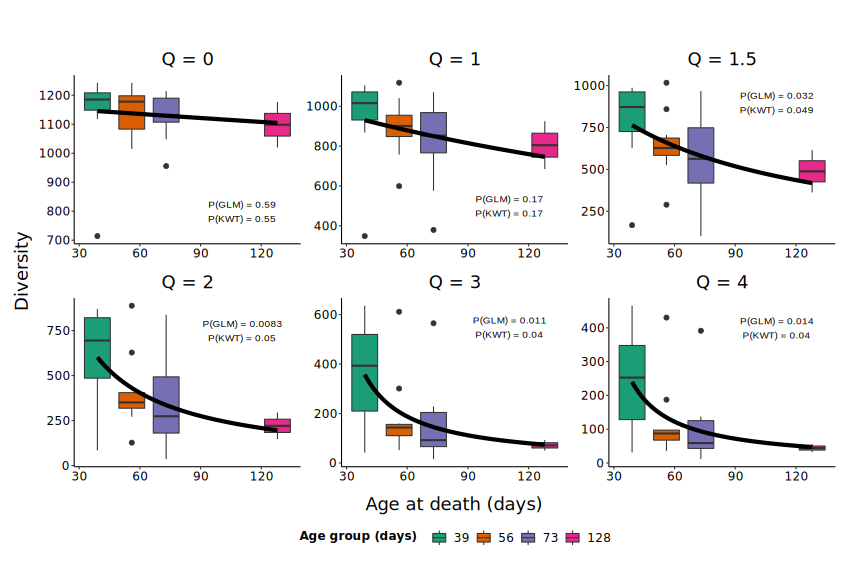
\includegraphics[width = 0.9\textwidth]{_Figures/png/ageing-clone-diversity-solo-fit-gamma}
\caption{Boxplots of Hill diversity values for the antibody repertoires of individuals of each age group in the \igseq ageing dataset at a sample of diversity orders, overlaid with the predictions of the best-fit Gamma-distributed generalised linear model at each order.  Annotated $p$-values indicate the statistical significance of the estimated age effect on diversity under the GLM ($P(GLM)$) and a Kruskal-Wallis test ($P(KWT)$) for each diversity order.}
\label{fig:igseq-ageing-clone-diversity-solo-fit-gamma}
\end{figure}
